\section{Linux namespaces}
\label{sec:intro:containerization:linux_namespaces}
A Linux namespace encloses a global system resource in an abstraction that makes the processes within the namespace appear to have their own isolated instance of the global resource \cite{ns}.
Changes to the global resource are visible to other processes that are members of the namespace but invisible to other processes.
Namespaces are the basic building block of containers under Linux. The following namespaces exist under Linux as the Linux kernel manual shows \cite{ns}.
\begin{itemize}
\item Cgroup
\item Interprocess communication (IPC)
\item Network
\item Mount
\item PID
\item User
\item UTS
\end{itemize}
Unfortunately it is utopic to describe every namespace type in depth in this work. 
First the IPC and mount namespace are described now briefly.
Later on the more interesting namespaces are explained in a dedicated subsection.

Mount namespaces provide an isolation of the list of mount points seen by the processes in each namespace instance.
Processes in each of the mount namespace instances see different single views of directory hierarchies.
This view can range from physical or network drives, mount paths or advanced features such as union file systems \cite{mountns}.

IPC namespaces isolate certain IPC resources like System V IPC objects and POSIX message queues which are both data structures that allow via shared memory to transfer information between processes \cite{ipcns}.

\subsection{PID}
\label{sec:intro:containerization:linux_namespaces:pid_namespaces}
Traditionally the Linux kernel has always maintained a single process tree. 
The tree contains a reference to each process currently running in a parent-child hierarchy. 
A Linux system starts with process PID1. 
This is the root of the process tree and the root process initiates the rest of the system by starting different handlers and services. 
All other processes start below this process PID1 in the tree. 

The basic idea behind PID namespaces is to create and append a new root tree to the already existing tree with its own PID1 \cite{pidns}. 
This makes the child process to a root process.
Processes in the subordinate namespace have no way to detect the existence of the parent process. 
This ensures that processes that belong to a process tree do not inspect or kill processes in other process trees. 
However processes in the higher-level namespace have a full view in the lower-level namespace of processes.

\subsection{Network}
\label{sec:intro:containerization:linux_namespaces:network_namespaces}
Due to the global instance of the network interface on a single host it is possible with granted permissions to alter routing and ARP tables. 
With network namespaces entirely different instances of network interfaces can be provided \cite{nwns}. 
Routing and ARP tables then operate independent of each other. 
This prevents communication between network namespaces.
 
Network namespaces are complex but important to know. 
These are responsible to establish communication between containers and hosts and between containers themselves. 
The following enumeration shows the standardized CNI (Container Network Interface) workflow \cite{Charles2013}. 
CNI describes how network namespaces are created and how a desired communication between these namespaces can be established.

\begin{enumerate}
\item Create network namespace
\item Create bridge network/interface
\item Create virtual-ethernet pairs
\item Attach virtual-ethernet to namespace and bridge
\item Assign IP addresses
\item Bring interfaces up
\end{enumerate}
For a better understanding an example with 2 network namespaces is shown in Figure \ref{sec:intro:containerization:linux_namespaces:netowork_ns}. 
Each color represents a network namespace with its associated virtual network interface pairs(veth-x and veth-x-bridge). 
For simplicity IP addresses are not shown. 

In this picture C1 is just a prefix for the underlying hostname. This hostname is arbitrary set. 
Basically communication between any networks from a view of a network namespace is not possible as already mentioned. 
Network communication between namespaces is allowed after the CNI procedure. 
Finally the two interface endpoints (purple and orange) have a valid IP address which leads to a working network communication.
\begin{figure}[htbp]
 \centering
 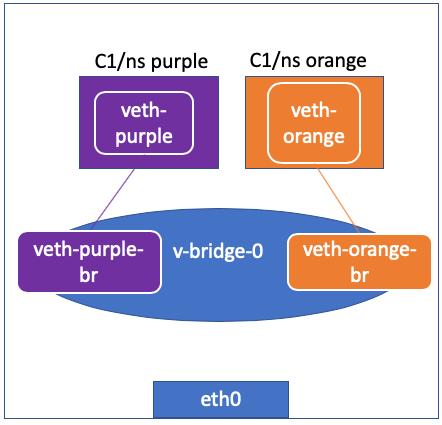
\includegraphics[width=0.4\textwidth]{gfx/examples/network_ns}
 \caption{Communication between network namespaces}
\label{sec:intro:containerization:linux_namespaces:netowork_ns}
\end{figure}
This is the beginning of network communication through namespaces and CNI. 
However only inter communication between different namespaces on a single host is not sufficient. 
Several steps are required to communicate externally to other host and across the internet.

Figure \ref{sec:intro:containerization:linux_namespaces:netowork_ns_out} displays a more comprehensive setup. 
It shows that the local host is also the gateway because it has one network connection through the interface eth0 and it has access to the bridge network created on the host. 
If the blue namespace network needs to access the endpoint with the IP address 192.168.1.3 a routing table entry in the blue network namespace like the following is necessary.
\begin{lstlisting}
	ip netns exec blue ip route add 192.168.1.0/24 via 192.168.15.5
\end{lstlisting}
This allows the direction from the namespace to the outside endpoint. To enable access from outside to this network namespace it is necessary to create a NAT rule via iptables.
\begin{lstlisting}
	iptables -t nat -A POSTROUTING -s 192.168.15.0/24 -j MASQUERADE	
\end{lstlisting}
In order to provide access to the internet from a namespace it is necessary to add a default route as seen below.
\begin{lstlisting}
	ip netns exec blue ip route add default via 192.168.15.5
\end{lstlisting}
\begin{figure}[htbp]
 \centering
 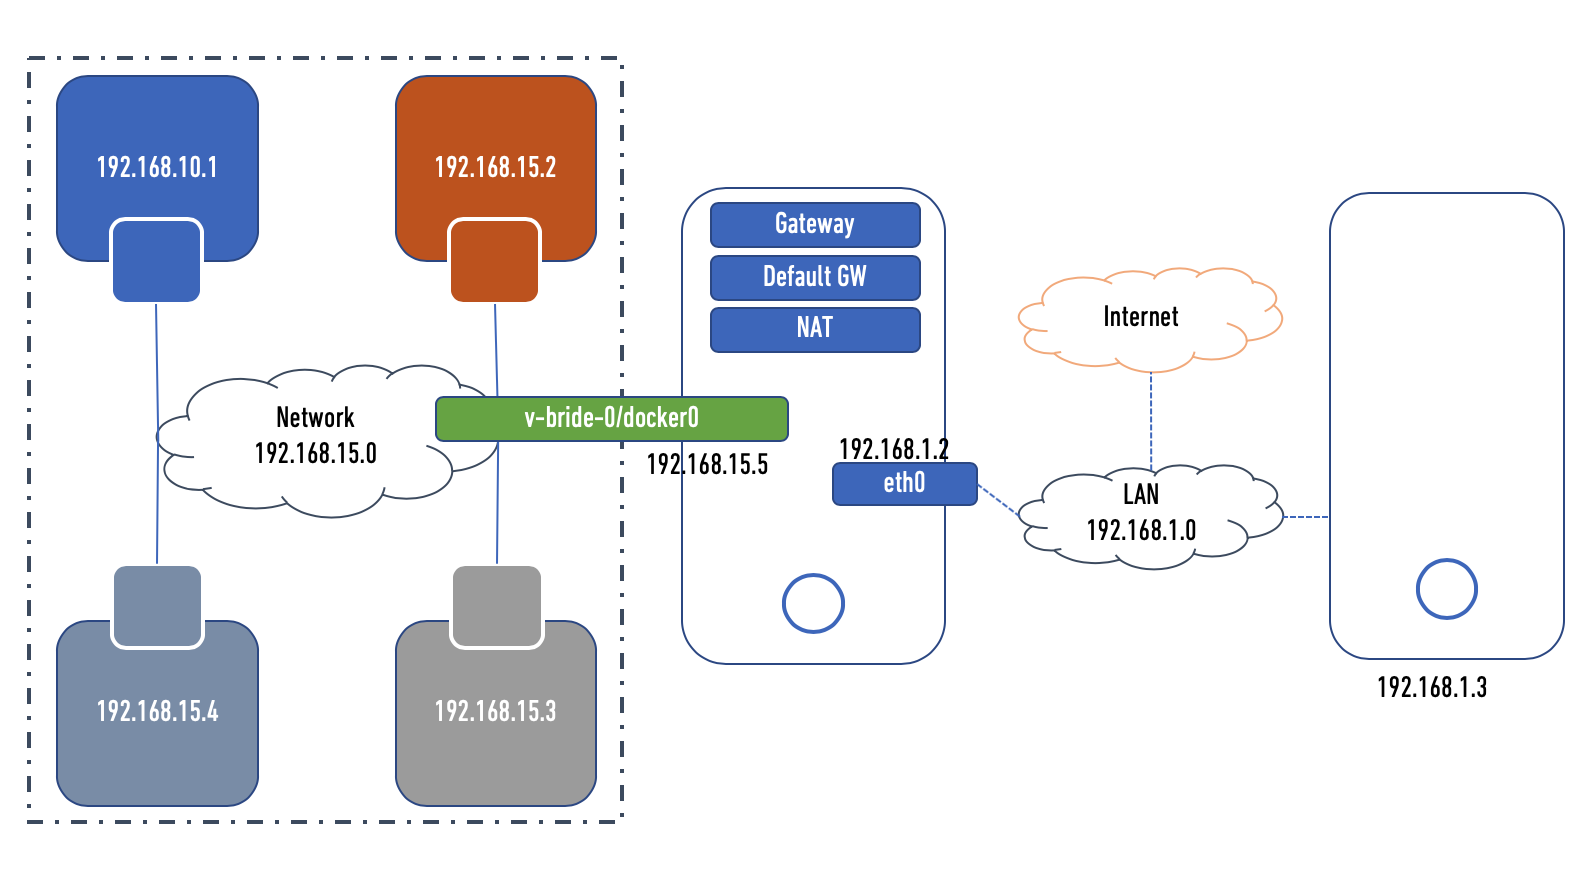
\includegraphics[width=0.7\textwidth]{gfx/examples/network_ns_out}
 \caption{Communication across network namespaces}
\label{sec:intro:containerization:linux_namespaces:netowork_ns_out}
\end{figure}
This example of network namespaces demonstrates the power and flexibility of network namespaces.
Normally these steps are automatically done through a container daemon like Docker. This in turn can also be managed by an orchestrator like Kubernetes or Mesos.

Lastly the user namespace is left and described in the following.

\subsection{User}
\label{sec:intro:containerization:linux_namespaces:user_namespaces}
User namespaces isolate user and group IDs so that they appear differently in and outside the user namespace.
Also they give processes the ability to believe that they are working as root when they are inside the namespace.
User namespaces can also operate on capabilities. 

But What are capabilities? In contrast to privileged processes that bypass all kernel permission checks unprivileged processes have to pass full permission checking based on the processes credentials such as effective UID, GID and supplementary group list. 
Linux has privileged process rights divided into different units called capabilities. These distinct units/privileges can be independently assigned and enabled for unprivileged processes \cite{capa}.

The next section briefly describes in short another Linux kernel feature called cgroups. 
They provide another level of security in order to contribute to a smooth working container environment.

\section{Cgroups}
\label{sec:intro:containerization:cgroups}
Control groups (Cgroups) are a way of enforcing hardware resource limitations and access controls on a process or set of processes. 
The cgroup scheme provides a hierarchical, inheritable and optionally nested resource control mechanism.
In the world of containers Cgroups are mandatory to prevent runaway containers and denial of service attacks.
The following enumeration contains the resources that are controlled by cgroups as listed in the Linux manual \cite{capa}.
\begin{itemize}
\item CPU usage
\item Memory usage
\item Disk usages
\item Device whitelist
\item Network traffic based on tags(class id values) and iptables for filtering
\item Application freeze and unfreeze by sending special signals
\item PID limitation to limit a specific amount of processes 
\end{itemize}

Now awareness is raised that containers work in isolation via native Linux functions.
The next important section gives an architectural introduction to the base of every container image - an union file system.
